\documentclass[a4paper,12pt]{article}

\usepackage[margin=2.75cm]{geometry}
\usepackage{lipsum}
\usepackage{libertine}
\usepackage{multirow}
\usepackage{makecell}
\usepackage{tabularx}
\usepackage{graphicx}
\usepackage{soul}
\usepackage{xcolor}
\usepackage{booktabs}
\usepackage{amsmath}
\usepackage[colorlinks=false, pdfborderstyle={/S/U/W 1}]{hyperref}

\usepackage{fontspec}
\setmonofont{Courier New}

\usepackage[backend=biber, 
natbib=true, 
style=C:/texmf/bst/biblatex-sp-unified/bbx/biblatex-sp-unified,
citestyle=C:/texmf/bst/biblatex-sp-unified/cbx/sp-authoryear-comp, 
maxbibnames=99, 
isbn=false, 
doi=false, 
eprint=false]{biblatex}
\addbibresource{ep.bib}

\usepackage[libertine]{newtxmath} % to get libertine as math font too

\usepackage{xspace}

\usepackage{enumitem}
%\setlist{nosep}
\setlist{noitemsep}

\usepackage{url}
%\urlstyle{same}

\usepackage{setspace}
\onehalfspacing

%\pagenumbering{gobble}

% ------------------------------------------------------------------------------------------------------ %

\begin{document}

\noindent PM1 Question Processing \hfill \today

\section*{Project plan: 20 Questions}
\noindent Wellesley Boboc, Anna-Janina Goecke, Rodrigo Lopez Portillo Alcocer, Elizabeth Pankratz

\subsection*{Task and motivation}

Our task is to build a system that will play the game 20 Questions (20Q).
A human player will be able to think of a target object, and the system will strategically questions that allows it to narrow down the candidate objects in its knowledge base.
It will incorporate the answers it receives and ultimately make a guess about what that target object could be.
If the target object is not already in its knowledge base, it will be added in based on the information the user has provided, probably interpolating from other closely-related objects.

This task is interesting and challenging, because it not only involves generating natural-language questions to present to the human player, but also choosing which questions are the best ones to ask, and manipulating the knowledge representation in accordance with the answers that the human player provides.

So, on the one hand, the project contains the computational-linguistic subtask of question generation (given a feature in the dataset, generate a natural-language question asking about that feature to display to the user), and on the other the engineering subtask of knowledge base manipulation.
There, we will need to strategically select the best question to ask, incorporate the answers from the user as the game is played, and at the end, add previously-unseen objects into the knowledge base.

\subsection*{Related work}

\hl{TODO: What work are you building on (= papers you read)?  What have they done? How do they define the problem? Is this a good kind of definition? What do you approach differently from them / how do you go beyond?}

We could take inspiration from literature on 20Q overall (there have been RL approaches, what else?) as well as from literature on rule-based question generation.

\subsection*{Data}
We are currently developing the implementation on a preliminary knowledge set available \href{https://github.com/drdevinhopkins/20_Questions/blob/master/knowledge_base.csv}{here}.
It is a table consisting of 100 objects (mostly animals) and 28 features for each, and each cell in the table is populated with a 1 or a 0 to indicate that the given animal does or does not have the given feature.
For example, the first few rows and columns of the dataset look like this:

\begin{center}
	\begin{tabular}{lcccccc}
	\toprule
Animal & Hair & Feathers & Eggs & Milk & Airborne & \ldots \\ \midrule
aardvark & 1 & 0 & 0 & 1 & 0 & \ldots \\
antelope & 1 & 0 & 0 & 1 & 0 & \ldots \\
bass & 0 & 0 & 1 & 0 & 0 & \ldots \\
bear & 1 & 0 & 0 & 1 & 0 & \ldots \\
boar & 1 & 0 & 0 & 1 & 0 & \ldots \\
\vdots & \vdots & \vdots & \vdots & \vdots & \vdots & $\ddots$ \\
\bottomrule
\end{tabular}
\end{center}

Whichever dataset we end up actually using must be larger than this and have many more features.
We are currently looking for open-source knowledge bases like this to use.

%What data would you use (where is the data/annotation available? What is annotated in the data, how big is it? What is in there, etc)

\subsection*{Implementation}

The machine learning system that we will use to implement this task is fairly simple: we will just use a decision tree (DT).
It is intuitive to think of 20Q as a DT, where asking/answering each successive question ``prunes the branches'' until (in a perfect world) there is only one leaf node remaining, representing an object that has all the properties specified by the player.
This is why we have chosen this approach.
Also, it is appropriate for smaller datasets, and since we don't know yet what kinds of knowledge bases are available, we wanted to have a system that is as flexible as possible.

The steps in our implementation will be as follows (everything following 1 can be concurrent):
\begin{enumerate}
	\item Write baseline DT system that decides at each step the optimal question to ask, narrows down the knowledge base to the objects compatible with the yes/no answers it receives, and ultimately makes guesses until the number of questions has reached 20 (we've pretty much finished this already).
	\item Incorporate handling of answers beyond yes and no.
	\item Implement the rule-based question generation, based on the structures of yes/no questions in corpora, e.g.\ Switchboard.
	\item Implement the incorporation of previously-unseen objects into the knowledge base.
\end{enumerate}


\hl{So, how do we choose which question to ask at any given time?
We use the principle of information gain.
[...]}

There are certainly other ways to choose a question.
One could also make this more complex by learning from previous games, performing an analysis of the features to see which ones are mutually exclusive, and so on.
But we're keeping it simple for now.


\subsection*{Evaluation}

There is a straightforward measure of success of our system overall: $\frac{\text{games won}}{\text{games played}}$. But because the system will consistently improve as we add new objects to its knowledge base, the success rates we get in early games with the system will presumably not be as good as success rates from later games. We can track this in a sort of growth curve across games:
	
\begin{center}
	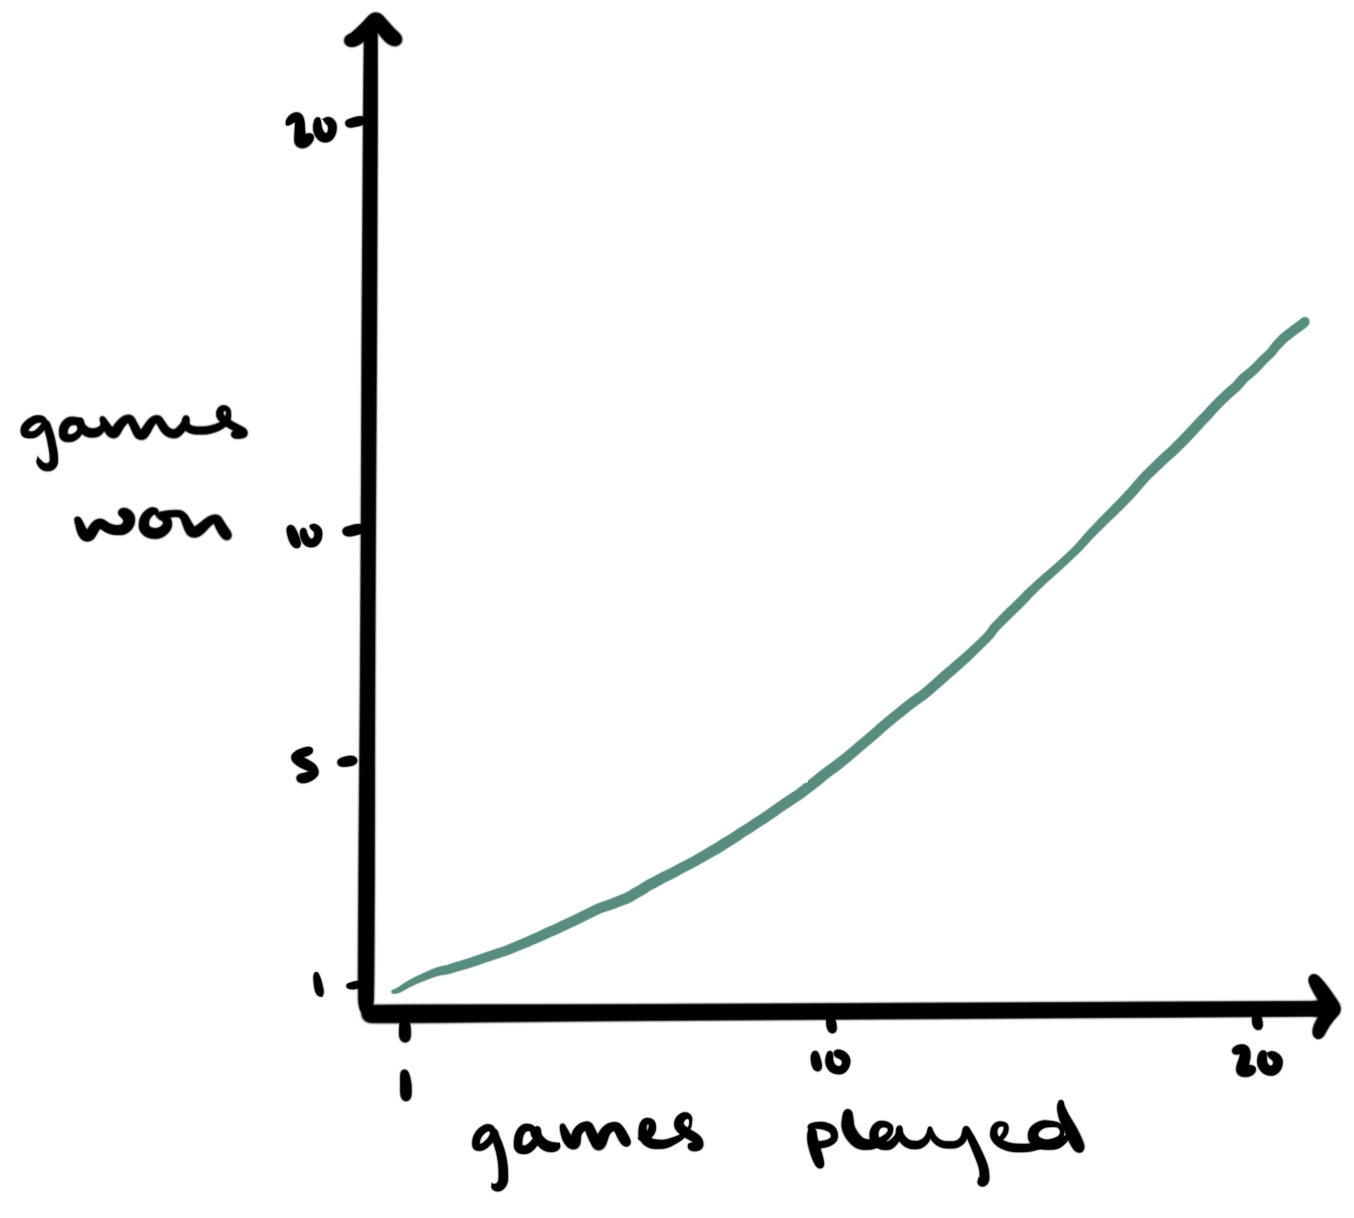
\includegraphics[width=.5\linewidth]{growth-curve.png}
\end{center}

The slope of the curve won't ever get bigger than one, but we'd want it to approach one, since that means the system is winning every game that it plays.
The slope of that curce at its endpoint is actually given by the rational expression $\frac{\text{games won}}{\text{games played}}$ \citep{Baayen2001}, so we can evaluate how our system performs after $x$ games by looking at how close that value is to 1.

Alternately, we could look at $\frac{\text{games lost}}{\text{games played}}$ and see how close that value gets to zero.

\begin{center}
	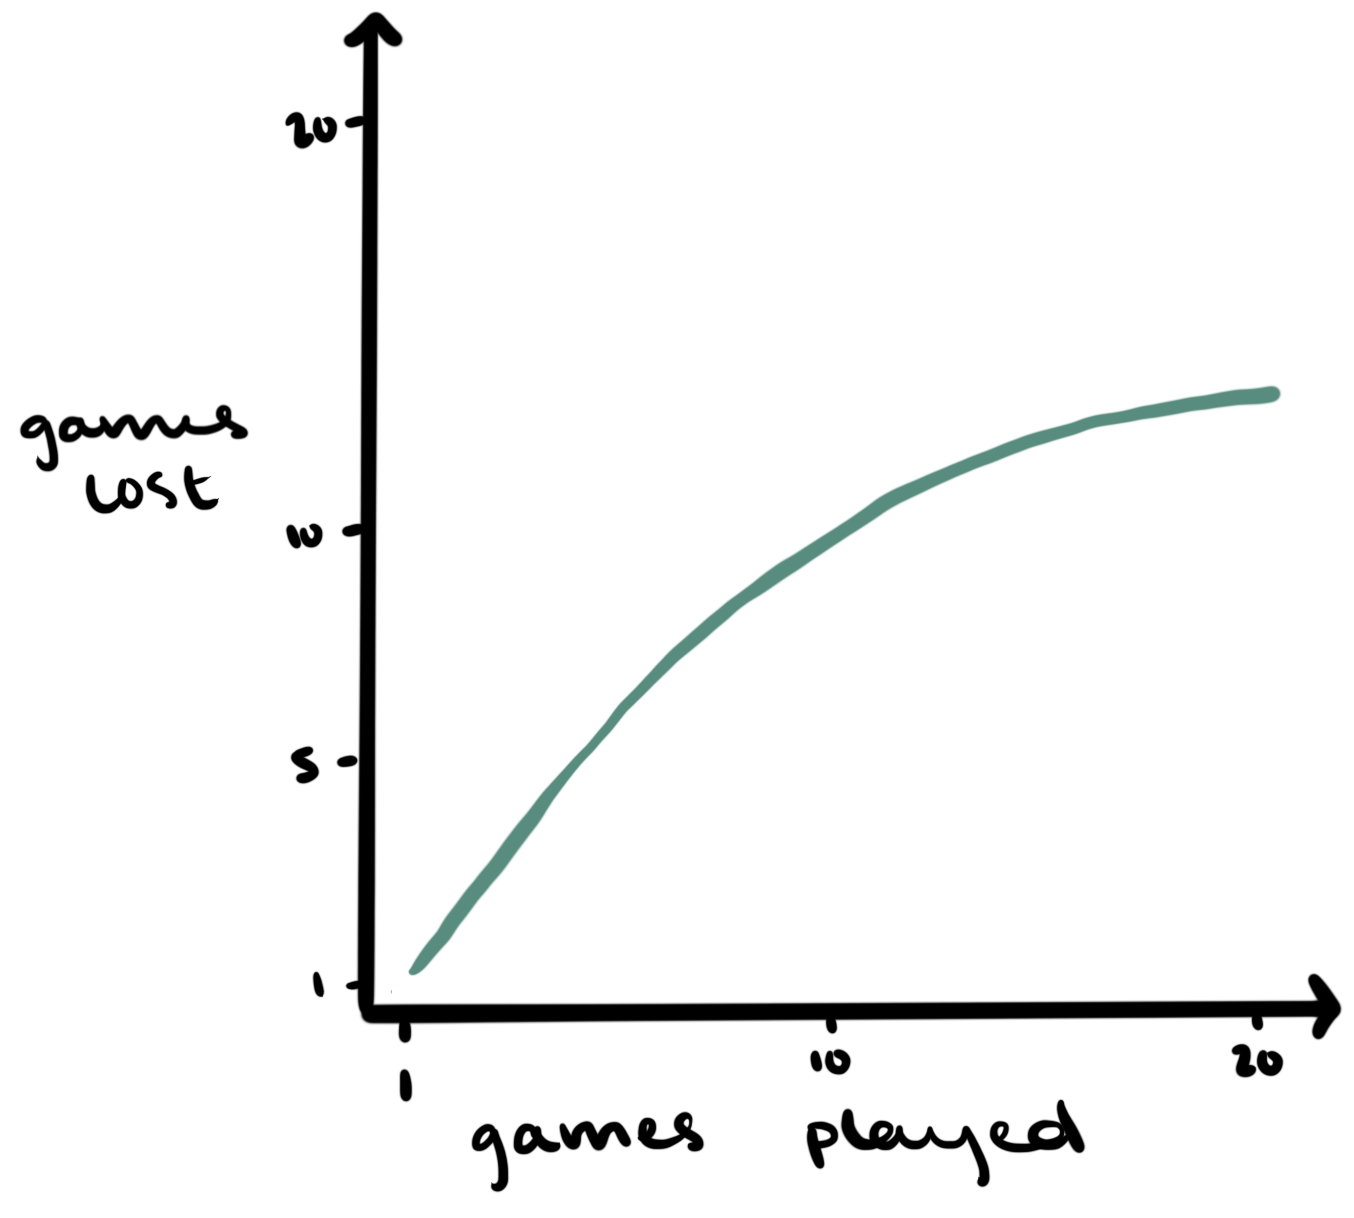
\includegraphics[width=.5\linewidth]{growth-curve2.png}
\end{center}

(We should also keep track of whether/how many losses come from exceeding the 20 question limit and how many come from out-of-database items. Ideally, the 20-question-limit curve will not change much, and the out-of-database curve would change more.)

Also, we should evaluate the goodness of the out-of-database items that we interpolate.
We could use human annotators who don't look at any of the other items in the dataset and only annotate the out-of-database items for all the features we use? 
Then we can compare their results to those output by Rodrigo's system. 
(We could either do it ourselves or source some ``crowdworkers'' among our friends using Google Forms again---will leave this up to Anna and/or Wellesley).

% -----------------------------------------------
\singlespacing
\printbibliography
% -----------------------------------------------

\end{document}